%!TEx root = ../physical-olympics-2.tex
\chapter{流体}



\section{流体的物理描述}

我们暂时只研究流体的动力学特征.\,规避掉任何有关热学的问题.

首先考察流体的运动学.\,流体已经不再具有恢复任何形变的能力,\,故引入流体相对初始时刻的位移已经不是最合适的方法了.\,如果依然这么处理,\,把流体质元的位置写为初始位置和时间的函数,\,这个描述方法称作\emph{拉格朗日法}(Lagrange's method).\,即:
\[\bs{r}=\bs{f}(\bs{R},\,t)\]

这样我们自然地可以得到一条曲线和它的方程,\,便是选定某个$\bs{R}=\bs{R}_0$,\,于是位置$\bs{r}$单独成为某个时间的函数.\,这代表某个质元的实际运动过程和轨迹.\,这个轨迹称作\emph{迹线}(path line).

但是,\,跟常见的做法是,\,我们不再关心每一个时刻各个空间位置的质元的初始位置在哪儿,\,这没有太大的意义.\,值得关心的当下流体在做何种流动.\,即每一个点处的流速$\bs{v}(\bs{r},\,t)$是如何的.\,其实就是上面函数的对时间偏导数:
\[\bs{v}(\bs{r},\,t)=\left.\frac{\partial \bs{f}}{\partial t}\right|_{\bs{R}:\,\bs{f}(\bs{R},\,t)=\bs{r}}\]

\begin{wrapfigure}[10]{o}[-10pt]{7cm}
\vspace{-0.1cm}
\centering
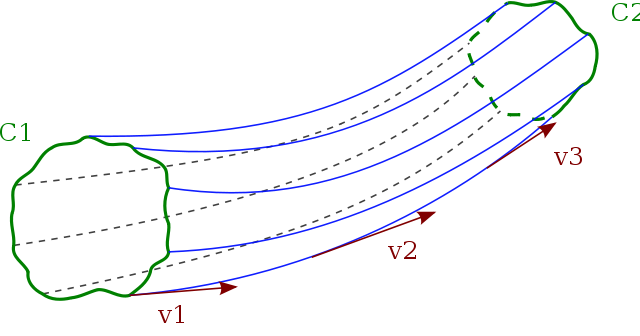
\includegraphics[width=7cm]{image/6-8-1.png}
\caption{流线与流管}
\end{wrapfigure}
用流速场$\bs{v}(\bs{r},\,t)$来描述流体的方法称作\emph{欧拉法}(Euler's method).\,而欧拉法的抽象函数也可以可视化:\,我们找到这样的空间曲线,\,数学上称作流速场的积分曲线:\,它在每一点的切线方向与某一时刻$t_0$下该点流速相同,\,或者说它是以下微分方程的解:
\[\frac{\ud x}{v_x|_{t=t_0}}=\frac{\ud y}{v_y|_{t=t_0}}=\frac{\ud z}{v_z|_{t=t_0}}\]

这样的曲线就叫\emph{流线}(streamline),\,一组流线还可以形成\emph{流管}(streamtube)的概念.\,流线与迹线显然不一定重合,\,因为流线只需要给出某一时刻的流速场就可以画出来,\,但迹线显然是要追踪不同时刻一个质元的运动,\,如果下一时刻的流速场变了,\,流体质元就会沿另一套流线去运动了.\,但即使迹线不再直观,\,使用欧拉法的优越性与完备性后面就会逐渐发现.

讨论流体的运动时有两个常见的特殊情况与条件可以使问题变得更简单:

一是,\,常见的液体,\,常常被建模为\emph{不可压缩流体}(incompressible fluid).\,它有两种等价的表述方式.\,一方面由于体积不可被压缩,\,质量又守恒.\,其密度便是个常数:
\[\rho={\rm Const.}\]

又或者关注流速场的性质就会发现,\,这个场只能是无散的,\,否则就会因为流体流向局域体积元造成内部质量增加:
\[\nabla\cdot \bs{v}=0\]

正因为这一点,\,液体作为流体的计算更简单,\,其结果也更简单:\,动力学的流动与热学往往是解耦合的,\,流体的温度分布在这个模型性不会影响到流体的运动,\,反过来流体的流动却必然对传热有影响.\,比如搅动冷热不均匀的水,\,水的运动几乎由搅动的方式决定而与温度分布有关,\,但水的温度变化显然受到搅动的强烈影响.\,但是在非常常见的\emph{对流传热}(heat transfer by convection)问题中,\,温度变化导致的密度变化产生的动力学效果是不可或缺的一环,\,那种场合就绝对不能把流体视作不可压缩流体.\,典型的情况,\,液体比如水锅烧水时的强对流情况,\,探究洋流的产生等等,\,气体则几乎都需要视作可压缩的流体.

可压缩的流体也存在质量的\emph{连续性方程}(continuity equation).\,我们可以把可变的密度$\rho$和流速$\bs{v}$相乘作为流密度矢量$\bs{j}$,\,那么:
\[\nabla\cdot(\rho \bs{v})+\frac{\partial \rho}{\partial t}=0\]

再注意到,\,$\bs{v}\cdot\nabla$这个算符其实就是跟随运动的流体一起运动,\,但是时间不变化,\,求物理量导数的算符,\,称为\emph{随体导数}(material derivative).\,它与在局部求时间的偏导算符$\partial/\partial t$,\,称作\emph{局部导数}(local derivative)之和就是跟随流体质元一起运动,\,还考虑时间的流逝情况下的完整导数,\,即\emph{全导数}(total derivative):
\[\frac{\uD}{\uD t}=\bs{v}\cdot\nabla+\frac{\partial}{\partial t}\]

通过这一点我们就把反映物质转移与质量守恒的连续性方程写成了以下更具有解释性的形式:
\[\rho \nabla\cdot \bs{v}+\frac{\uD \rho}{\uD t}=0\]

这意味着,\,流体速度场存在散度就会导致流体质元随运动发生密度变化.\,从而也把不可压缩流体满足的两个条件联系在了一起.

第二个特殊情况与条件是,\,如果流体的流速场不随着时间变化而仅仅是位置的函数:
\[\bs{v}=\bs{v}(\bs{r})\]

这样的流动就称为\emph{定常流动}(steady flow).\,否则称作\emph{非定常流动}(unsteady flow).\,定常流动的意义需要在本章过程中慢慢体会.\,目前已经能够发现一点:\,只有在定常流动情况下,\,流线与迹线才是彻底重合的.

下面类似于弹性体,\,我们把流体在某个代表点,\,不妨就设在原点$\bs{0}$,\,附近的$\bs{r}$处的流速场进行泰勒展开,\,保留到一阶:
\[\bs{v}(\bs{r})=\bs{v}(\bs{0})+\bs{r}\cdot \nabla \bs{v}\]

同理,\,把张量$\nabla \bs{v}$分解为对称部分和反对称部分:
\[\nabla \bs{v}=\bs{\varepsilon}+\bs{\omega}\]
\[\bs{\varepsilon}=\frac{\nabla \bs{v}+\phantom{}^{\rm t}\nabla \bs{v}}{2}\quad,\quad \bs{\omega}=\frac{\nabla \bs{v}-\phantom{}^{\rm t}\nabla \bs{v}}{2}\]

这样流体的运动就被分解为三个部分:
\[\bs{v}(\bs{r})=\bs{v}(\bs{0})+\bs{r}\cdot \bs{\omega}+\bs{r}\cdot \bs{\varepsilon}\]

最后一项尤其值得注意,\,前两项表示流体跟随中心整体的平动和绕中心的转动,\,质元与质元之间本质是没有相对运动与变形的.\,第三项就表示会不可避免地产生质元与质元相对摩擦的情况.\,它由对称张量$\bs{\varepsilon}$描述.\,与弹性体的应变张量相似却又不同,\,这里不是位移而是速度作为了变量去求导.\,称作\emph{应变率张量}(rate-of-strain tensor):
\[\bs{\varepsilon}=\begin{bmatrix}\frac{\partial v_x}{\partial x}&\frac{1}{2}\frac{\partial v_y}{\partial x}+\frac{1}{2}\frac{\partial v_x}{\partial y}&\frac{1}{2}\frac{\partial v_z}{\partial y}+\frac{1}{2}\frac{\partial v_y}{\partial z}\\\frac{1}{2}\frac{\partial y}{\partial x}+\frac{1}{2}\frac{\partial v_x}{\partial y}&\frac{\partial v_y}{\partial y}&\frac{1}{2}\frac{\partial v_x}{\partial z}+\frac{1}{2}\frac{\partial v_z}{\partial x}\\\frac{1}{2}\frac{\partial v_z}{\partial y}+\frac{1}{2}\frac{\partial v_y}{\partial z}&\frac{1}{2}\frac{\partial v_x}{\partial z}+\frac{1}{2}\frac{\partial v_z}{\partial x}&\frac{\partial v_z}{\partial z}\end{bmatrix}\]

最后还需要描述流体中的力.\,用应力张量来描述流体中的受力情况是合适地.\,但是我们发现问题可以进一步简化.\,首先我们考虑一种更简单的情况:\,\emph{流体静力学}(hydrostatics).

我们知道,\,在流体中没有静摩擦的可能性.\,流体中的摩擦,\,即\emph{湿摩擦}(wet friction),\,只有可能是静摩擦.\,这是因为流体没有保持初始形态的能力,\,它只有一定的保持体积的能力,\,故对于不改变体积的剪应变,\,顶多只能阻碍,\,但不能恢复.\,故一个流体在剪应力下应当马上运动起来,\,不可能处于静止状态.\,故流体静力学必然只能处于正应力下,\,而且沿不同方向的正应力还必须相等,\,否则在不同坐标系下就有可能产生剪应力.\,这实际上就证明了我们熟悉的流体静力学内应力由标量\emph{压强}(pressure)来描述的观点,\,注意正应力以拉力为正,\,压强对应负的正应力:
\[\bs{\sigma}=-p\bs{I}\]

那么计算一个体积区域$V$边界$\partial V$上的压力合力,\,可以由高斯定理得到:
\[\bs{F}=\oint\limits_{\partial V}\ud \bs{S}\cdot \bs{\sigma}=-\oint\limits_{\partial V}p\ud \bs{S}=\int\limits_{V}\nabla\cdot\bs{\sigma}\ud V=-\int\limits_{V}\nabla p\ud V\]

这样就计算出来了内应力造成的体积力:
\[\frac{\ud\bs{F}}{\ud V}=-\nabla p\]

例如在重力场中的水$\nabla p=\rho \bs{g}$为常矢量,\,那么对没入水中的体积造成的浮力就是:
\[\bs{F}=-\int\limits_{V}\nabla p\ud V=-\int\limits_{V}\rho \bs{g}\ud V=-\rho \bs{g}V\]

这就是古希腊时期就被发现的著名的\emph{阿基米德原理}(Archimedes' principle),\,今天看来它等价于高斯定律和尚未证明但正确的$\nabla p=\rho \bs{g}$.\,这个式子其实就是平衡方程.\,设想处于平衡状态的静力学流体还受到外力场,\,体积力为$\bs{f}(\bs{r})$.\,那么为了平衡就需要满足:
\[\nabla p=\bs{f}\]

马上就可以发现,\,这个式子一方面作为了压强分布的计算公式,\,同时,\,也由于左侧是一个标量场的梯度,\,在闭合路径上的积分必然给出零的结果,\,它又等于右侧,\,我们等于证明了:\,只有在外保守力场下的流体系统才有可能处于平衡状态.

\vspace{0.5cm}

那么,\,当流体开始运动起来,\,此时继续用压强描述流体内部应力就不再合适了,\,此时与上一章弹性体相同的是,\,我们可以引入对称的应力张量来修正原来的压强对应的单位张量:
\[\bs{\sigma}=-p_0\bs{I}+\begin{bmatrix}\sigma_{x}&\tau_{xy}&\tau_{zx}\\\tau_{xy}&\sigma_{y}&\tau_{yz}\\\tau_{zx}&\tau_{yz}&\sigma_{z}\end{bmatrix}\]

但仍然有一点值得注意,\,如果$\sigma_x,\,\sigma_y,\,\sigma_z$同时增加一个量,\,这和改变了$p_0$没有本质区别,\,所以我们希望压强$p_0$反映了正应力的平均效应,\,故调整前后的配比使得后面的张量称为无迹的张量$\bs{\tau}$,\,称为\emph{黏滞应力张量}(viscous stress tensor)或\emph{偏应力张量}(deviatoric stress tensor):
\[-p_0\bs{I}+\bs{\tau}\]
\[\bs{\tau}=\begin{bmatrix}\tau_{x}&\tau_{xy}&\tau_{zx}\\\tau_{xy}&\tau_{y}&\tau_{yz}\\\tau_{zx}&\tau_{yz}&\tau_{z}\end{bmatrix}\quad(\tau_{x}+\tau_{y}+\tau_{z}=0)\]

针对黏滞应力张量是否会产生,\,即流体有没有\emph{黏性}(viscosity).\,我们又可以找到一种特殊的情况:\emph{无黏性流体}(inviscid fluid),\,实际上经常被定义为\emph{理想流体}(ideal fluid).\,此时流体即使在动,\,其应力也只有压强.\,反过来就是需要考虑黏滞的\emph{黏性流体}(viscous fluid).



\section{定常流动动力学}

本节讨论范围仅限于无黏性流体.\,前半部分结论对于普遍的可压缩,\,非定常流体都是完全正确的.

若想为流体找到一个动力学方程,\,其实我们几乎已经在上一节完成了一大半.\,由于没有黏滞,\,上一节计算的内力的合力结果为:
\[\frac{\ud\bs{F}}{\ud V}=-\nabla p\]

再加上外体积力$\bs{f}$,\,现在要做的只不过是把上一节的平衡方程改成质元的牛顿定律,\,注意其中的加速度,\,应该用跟随质元一起运动而计算的全导数:
\[\rho \frac{\uD \bs{v}}{\uD t}=-\nabla p+\bs{f}\]

这就已经是能充分地解决问题的,\,流体需要符合的动力学方程.\,它被称作\emph{欧拉方程}(Euler equation).

另一个高频使用的方程是,\,如果我们再加上定常流动和不可压缩流体的限制条件,\,这就会导致著名的\emph{贝努力方程}(Bernoulli equation).\,暂时我们只加上定常流动这一个条件

\begin{figure}[H]
\centering
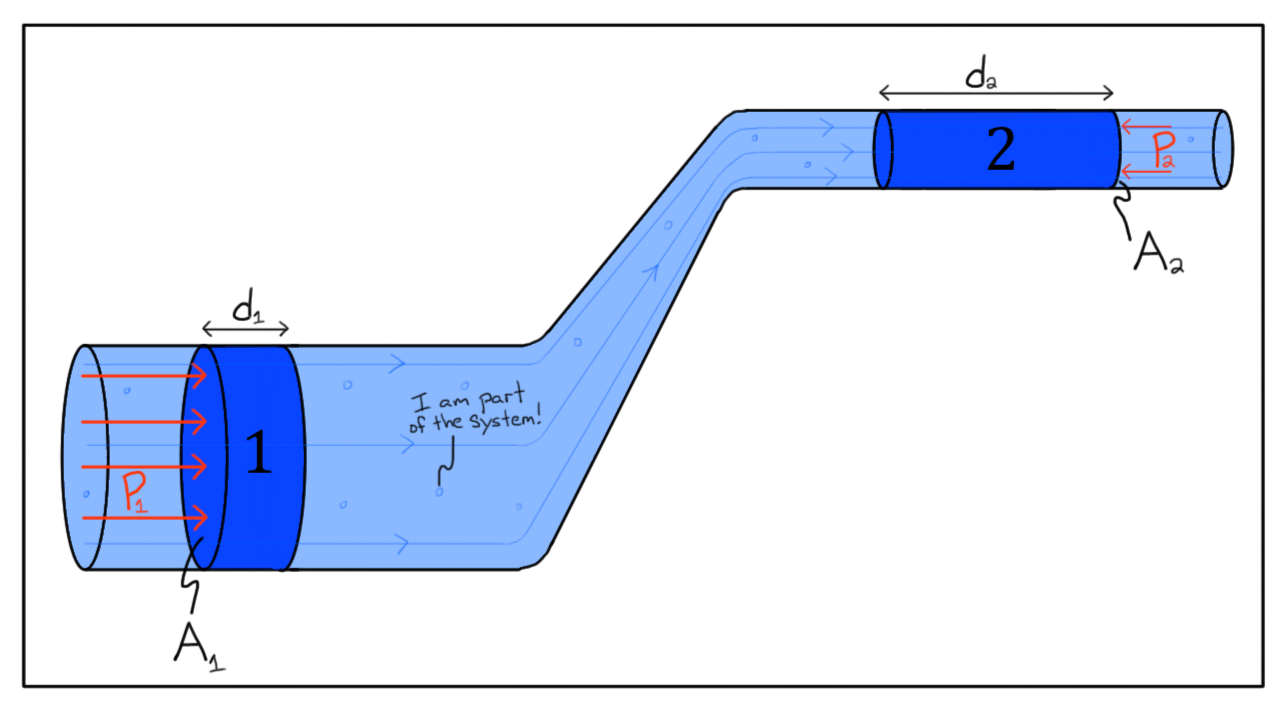
\includegraphics[width=14cm]{image/6-8-2.png}
\caption{贝努力方程}
\end{figure}

我们找到一根流线,\,并找到流线上的两个点$1$,\,$2$,\,在流线上垂直于流速方向把流线扩充为流管.\,那么在两处的面积$A$,\,和密度$\rho$就要满足连续性方程,\,这对应着\emph{流量}(flux)的不变性:
\[Q=\rho_1v_1A_1=\rho_2v_2A_2\]


将外体积力写作质量势$\varphi$的梯度$\bs{f}=-\rho\nabla \varphi$.\,写出定常流动下的欧拉方程:
\[\bs{v}\cdot\nabla \bs{v}=-\frac{\nabla p}{\rho}-\nabla \varphi\]

如果计算以下量的梯度:
\[\nabla\left(\frac{v^2}{2}+\frac{p}{\rho}+\varphi\right)=\bs{v}\times(\nabla \times\bs{v})+\bs{v}\cdot\nabla \bs{v}+\frac{\nabla p}{\rho}-\frac{p}{\rho^2}\nabla\rho+\nabla \varphi\]

借助欧拉方程,\,上式三项互相抵消,\,仍然剩下两项.\,但是现在我们在考察左侧标量在同一条流线上的表现,\,两侧点乘$\bs{e}_v$,\,右侧叉乘项由于垂直也消失:
\[\frac{\ud}{\ud s}\left(\frac{v^2}{2}+\frac{p}{\rho}+\varphi\right)=-\frac{p}{\rho^2}\frac{\ud \rho}{\ud s}\]

这说明我们得不到一个沿着流管守恒的量.\,事实上,\,$-\frac{1}{\rho^2}\frac{\ud \rho}{\ud s}$项其实就是$\frac{\ud }{\ud s}\frac{1}{\rho}$,\,即单位质量的物体具有体积沿着流线的变化率,\,那么它再乘以压强,\,就表示由于体积增加导致的对外界做功而减小的内部能量\footnote{还需要绝热条件,\,这样内能改变就只和做功有关.}:
\[-\frac{p}{\rho^2}\frac{\ud \rho}{\ud s}=-\frac{\ud u}{\ud s}\]

这样就得到了可压缩流体的贝努力方程:
\[u+\frac{v^2}{2}+\frac{p}{\rho}+\varphi={\rm Const.}\]

通过这一点可以发现,\,可压缩流体的内能往往是与动力学耦合在一起的,\,而内能又往往影响温度.\,所以内能的改变又会导致热学与动力学的耦合,\,问题就变得很复杂.

但是如果流体不可压缩,\,那么上式等号右侧$\rho$就是个常数,\,从而直接左侧就具有零的导数.\,那么我们就得到了不可压缩流体的贝努力方程,\,往往写作:
\[\frac{\rho v^2}{2}+p+\rho\varphi={\rm Const.}\]

\section{黏滞流体动力学}

\begin{wrapfigure}[10]{o}[-10pt]{7cm}
\vspace{-0.1cm}
\centering
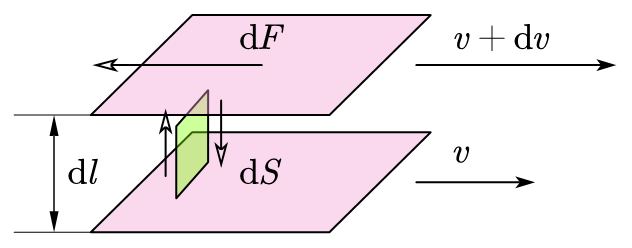
\includegraphics[width=7cm]{image/6-8-3.png}
\caption{牛顿黏滞定律}\label{6-8-3}
\end{wrapfigure}
描述黏滞流体的最标准的模型是\emph{牛顿流体}(Newtonian fluid)模型.\,核心的定律称作\emph{牛顿黏滞定律}(Newtonian law of viscosity).\,如图\ref{6-8-3}.\,如果流体速度场是完全单向的,\,且其大小的改变$\ud v$也只在垂直流速方向移动$\ud l$时发生,\,那么就定义流速梯度为:
\[2\varepsilon=\frac{\ud v}{\ud l}\]

而由此产生的切应力就是:
\[\tau=\frac{\ud F}{\ud S}\]

牛顿定律指出,\,两者应当成正比,\,比例系数就是\emph{黏滞系数}(viscosity),\,常简称黏度$\eta$.\,其单位是${\rm Pa\cdot s}$:
\[\tau=\eta\cdot 2\varepsilon\]

其实这里的黏度是\emph{动力学黏度}(dynamic viscosity)的简称.\,实用中常常遇到需要把它除以介质密度的情况,\,所以还有\emph{运动学黏度}(kinematic viscosity)的定义,\,其单位是${\rm m^2/s}$,\,与扩散系数单位是一样的:
\[\nu=\frac{\eta}{\rho}\]

显然,\,当我们考虑把牛顿黏滞定律进行推广时,\,第一个值得注意的现象就是,\,首先如果把流速方向记做$x$方向而变化方向记做$y$方向,\,那么一是应力$\tau$其实就是作为了$x-y$平面上的剪应力,\,为了满足流体的力矩平衡,\,不仅对$x$方向的分界面会产生$x$方向的黏滞摩擦力,\,对$y$方向的分界面也同时会造成$y$方向的力以抵消这个效应,\,在上图中,\,总是左侧的液体对右侧的液体给向下的力,\,右侧则给左侧向上的力.

第二点是,\,显然下式不具有对称性:
\[\tau_{xy}=\eta\frac{\partial v_x}{\partial y}\]

如果是$v_y$在随$x$产生改变,\,上式就正确了,\,此时同样会产生剪应力.\,所以我们猜想如下式子是正确的:
\[\tau_{xy}=\eta\left(\frac{\partial v_x}{\partial y}+\frac{\partial v_y}{\partial x}\right)\]

事实上这也是牛顿黏滞定律唯一可能正确的推广形式.\,单凭借这个结论我们就能得到很多有意义的结果.\,这里直接不加证明地介绍其中的两个.\,一是圆柱管道内的液体流动的\emph{哈根-泊萧叶方程}(Hagen-Poiseuille equation).\,如果管道半径$R$,\,体积流量$Q$,\,那么在长为$l$的一段上形成流动需要的压强差为:
\[\Delta p=\frac{8\eta Ql}{\pi R^4}\]

第二个式子是球形物体在黏滞流体中的阻力公式.\,著名的\emph{斯托克斯定律}(Stokes law).\,如果球体半径为$R$,\,速率为$v$,\,那么阻力大小为:
\[F=6\pi\eta rv\]

普遍的情形下,\,之前介绍过的黏滞应力张量与应变率张量之间的关系,\,根据对称性的原理,\,与上一章类似地,\,就写作:
\[\bs{\tau}=2\eta\cdot \bs{\varepsilon}+\lambda {\rm Tr}(\bs{\varepsilon})\cdot \bs{I}\]

只不过在这里,\,由于$\bs{\tau}$的无迹性,\,$\lambda$没有别的选则,\,只能取$-2\eta/3$.\,这样就得到了黏滞流体的内力的决定性的方程.\,最后,\,类似于欧拉方程的方式进行推导,\,我们最终得到了一个方程:
\[\rho\frac{\partial \bs{v}}{\partial t}+\rho\bs{v}\cdot\nabla\bs{v}=-\nabla p+\eta\nabla^2\bs{v}+\frac{1}{3}\eta\nabla(\nabla\cdot\bs{v})+\bs{f}\]

这个方程就是著名的\emph{纳维-斯托克斯方程}(Navier-Stokes equation).\,$\bs{v}\cdot\nabla\bs{v}$项使得这个方程成为非线性的偏微分方程.\,它的求解是如此之难,\,以至于在2000年它成了7个\emph{千禧年难题}(Millennium Prize problems)之一,\,而且仅仅是为了解决最最初步的问题:\,解的存在性与光滑性.\,第一个解决它的科学家将获得一百万美元的奖金,\,但目前这个问题的解决依然是遥遥无期的.




\section{*流体中的波}

\section{波的色散}